% Kepler --- arXiv submission source
\documentclass[11pt]{article}

\usepackage[utf8]{inputenc}
\usepackage[T1]{fontenc}
\usepackage{lmodern}
\usepackage{microtype}
\usepackage[margin=1in]{geometry}
\usepackage{amsmath}
\usepackage{booktabs}
\usepackage{graphicx}
\usepackage{array}
\usepackage[numbers]{natbib}
\usepackage[colorlinks=true,linkcolor=blue,citecolor=blue,urlcolor=blue]{hyperref}

\title{Kepler: Separating Discovery from Execution on ARC-AGI-3}

\author{Wensen Wu\\
Independent\\
\texttt{contact@wensenwu.com}\\
\texttt{wensenwu.com} $\cdot$ \texttt{github.com/Cveinnt}}

\date{}

\begin{document}

\maketitle


\begin{abstract}
Agent harnesses now report 99-class scores on ARC-AGI-3's public set, but results are difficult to compare because harnesses differ in \emph{what is scored}. We present Kepler, an open-source harness reaching a \textbf{server-verified exact 100.00} RHAE (Claude Opus 5, single configuration, all 25 games re-executed to 100 on the official replay) and 95.97 (GPT-5.6 Sol, also server-exact) on the public set: a 2,753-line system in which a frontier model builds and certifies an executable world model of each game, after which the harness---not the model---replays the certified solution as the scored attempt. We report four findings. First, mechanical replay of certified traces, rather than trusted live execution, accounts for the decisive gap between 99-class systems and the rest ($96.51 \to 98.86$ in our own ablation). Second, added discipline is not monotonically better: we publish a complete v1--v5 ablation, including a regression traced to enforcing a nonexistent official cutoff. Third, with execution largely saturated (43 of 50 game--model cells at 100 across two frontier models under one frozen harness), the benchmark's residual signal is discovery reliability. Fourth, a controlled modality ablation --- one flag switching text grids to rendered frames, all else fixed --- solved the one game six text-mode attempts had exhaustively ``proved'' unsolvable, in a single session: on such games the binding constraint is what the agent can perceive, not how it reasons. Every run ships as an append-only per-action ledger with adversarial audits---which twice caught integrity violations by our own agents---and every headline links its official replay scorecard, with every divergence disclosed.
\end{abstract}

\section{Introduction}\label{sec:intro}

ARC-AGI-3~\citep{arcagi3} evaluates an agent on unseen interactive games: a 64$\times$64 grid of 16 color indices, a set of legal actions, and nothing else --- no rule sheet, no object list, no stated goal, no shaped reward. Its metric, Relative Human Action Efficiency (RHAE), scores per completed level $\min((\texttt{human\_baseline}/\texttt{agent\_actions})^2,\, 1.15)$, weighted toward later levels, with a completion cap. It scores \emph{actions}, not tokens or wall-clock: an agent that thinks for an hour and then plays perfectly is rewarded; an agent that flails cheaply is penalized heavily.

Within months of release, harness-plus-frontier-model systems reported scores from 73.7 (a minimal 11-line scaffold) to 100.00 (Tycho). This spread is the interesting datum: the \emph{same class of models} spans 26 points depending on the process wrapped around them. But it also creates a credibility problem, because most of the spread lives in design decisions that are rarely stated: whether games are rerun on bad scores, whether the reported number is a best-of, whether the scored attempt was played live or replayed from a recording, and whether anyone audited the runs for the obvious failure --- an agent that found the answer rather than derived it. Greg Kamradt's criticism of the earliest ${\sim}$99\% claim (a per-game best-of-2 fallback rule, with score feedback: \emph{``the human and environment are injecting knowledge into the process''}~\citep{kamradt2026critique}) applies, in some form, to any published number whose selection and rerun rules are unstated --- including our own early ones.

Kepler is our answer to that problem: an independent implementation of the executable-world-model approach to this benchmark~\citep{tycho,thinharness}, evolved through eight published harness versions. Our approach is verification-first: we treat a self-reported score as credible only to the extent that it can be independently re-derived. Concretely:

\begin{itemize}
  \item \textbf{Single-configuration numbers are the headline.} One model, one frozen harness, one pass over all 25 games, no score-conditioned reruns. Best-of numbers are published only as a labeled capability ceiling.
  \item \textbf{Every run is published} --- the append-only per-action ledger, the agent's world model and notebook, failures and superseded runs included, with the reason for supersession.
  \item \textbf{Every headline is server-verified.} Each single-config number links an official ARC Prize scorecard produced by re-executing the recorded trace; divergences are disclosed, not absorbed (\S\ref{sec:matrix}).
  \item \textbf{The audits ran against us first.} The same adversarial tooling we ship caught our own agents twice --- once reading a game's source, once rebuilding the harness inside a control group --- and both incidents are published with evidence (\S\ref{sec:integrity}).
\end{itemize}

The paper's contributions are the four claims in the abstract, the harness itself (2,753 lines including the agent directive), and the published regression ladder --- which, to our knowledge, is the first ablation on this benchmark to report a negative result for added discipline mechanisms together with a diagnosis.

\begin{figure}[ht]
  \centering
  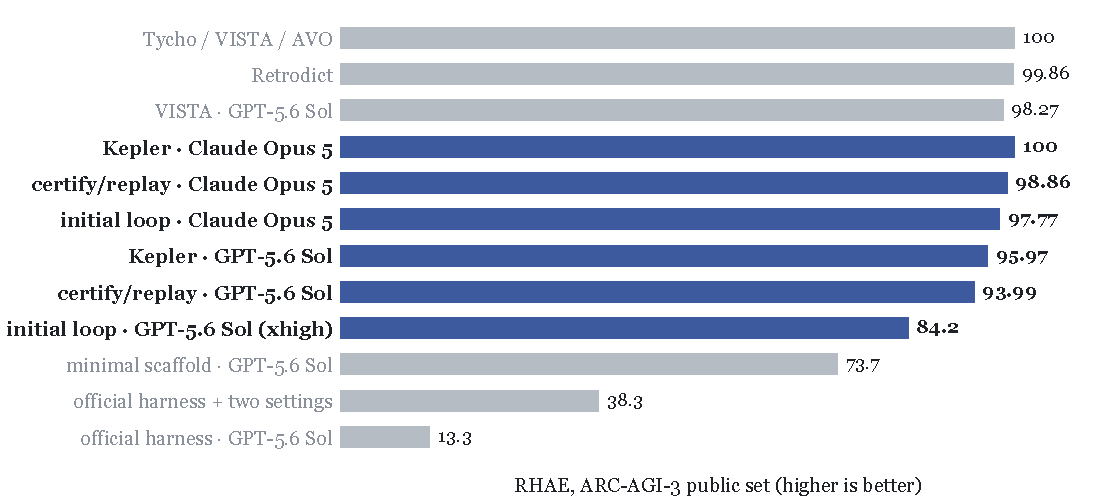
\includegraphics[width=\linewidth]{figures/fig1_ladder.pdf}
  \caption{The harness effect on ARC-AGI-3 (RHAE, public set). Gray: external systems as published; blue: Kepler single-configuration boards. The same model class spans 13.3--100 depending on the process wrapped around it; the systems at 100 --- ours included --- all score mechanically replayed traces rather than live play.}
  \label{fig:ladder}
\end{figure}

\section{Method}\label{sec:method}

\subsection{The loop: observe, model, certify, plan, commit}\label{sec:loop}

The agent is a stock CLI coding agent in a workspace. It never plays the game directly. The directive (\texttt{harness/directive.md}, 218 lines --- the entire ``prompt engineering'' of the system) frames the task as experimental physics: hypothesize the mechanism, encode it as an executable program, test it against recorded reality, and plan inside it.

Persistent state is three files. \texttt{world\_model.py} is the agent's theory of the game in two layers --- state grounding (named finders that turn pixels into objects) and mechanism (\texttt{simulate(grid, action)} written over those objects, not raw pixels). \texttt{notes.md} is a lab notebook with an epistemic discipline: every claim tagged \textbf{checked} (verified against the log) or \textbf{assumed}, and no multi-step plan built on assumed points. \texttt{events.jsonl} is the append-only timeline of every real transition ever taken --- ground truth the agent can read but not edit.

Five tools close the loop:

\begin{table}[ht]
  \centering
  \caption{The five workspace tools that close the loop.}
  \label{tab:tools}
  \begin{tabular}{@{}l p{0.55\linewidth} l@{}}
    \toprule
    tool & role & cost \\
    \midrule
    \texttt{observe.py} & read-only view of the current frame, diffs, per-level baselines & free \\
    \texttt{query.py} & compute over state instead of reading it (context thrift) & free \\
    \texttt{backtest.py} & replay \texttt{simulate} over the \emph{entire} recorded history; a theory that cannot retrodict the past does not get to predict the future & free \\
    \texttt{bfs.py} & plan inside the certified model (agents may also write their own searches) & free \\
    \texttt{commit.py} & the \textbf{only} channel to the real game & actions \\
    \bottomrule
  \end{tabular}
\end{table}

\subsection{The guarded channel}\label{sec:channel}

\texttt{commit.py} (508 lines) enforces prediction discipline mechanically: every committed action carries a prediction from the agent's own \texttt{simulate}; the action executes, and the first misprediction \textbf{voids the remainder of the plan} and returns the counterexample. This converts a wrong belief into a cheap, logged experiment instead of an expensive pile of wasted actions --- and it makes every committed plan a falsifiable statement of the model's current accuracy. Predictions may be partial (\texttt{None} for unclaimed cells --- a HUD strip, an animation region), but abstaining everywhere is rejected as vacuous. Three invariants hold the system up: reality outranks the model, history is append-only, and nothing reaches the game except through the predict-checked channel.

\subsection{Certify, then mechanically execute (v5)}\label{sec:v5}

RHAE scores the final full attempt --- the segmentation our verifier and the official replay both use --- so the winning shape of a game is learn (unscored: superseded by the attempt that follows), then speedrun (scored, minimal actions). Versions v1--v3 trusted the live agent to execute the speedrun it had certified. v5 removes the agent from the scored attempt entirely: the agent's job ends at writing \texttt{cleanrun.json} --- the full per-level action programs. \texttt{harness/ws\_tools/cleanrun.py} (176 lines, copied into each workspace as \texttt{tools/cleanrun.py}) then self-certifies the artifact (per-level program lengths within 1.3$\times$ the human baseline; each program simulated to \texttt{level\_up}/\texttt{win} from \emph{recorded} level-start grids when the world model exposes the threaded-state API; absent that API, certification degrades to length checks alone, a weaker guarantee we state rather than hide) and replays it through the daemon, halting on the first cell where the real game falsifies the model. The runner drives up to three certify+execute repair cycles; repairs can only fail closed. The scored attempt is thus a mechanical replay of a certified program --- the same architecture we found, by code diff, in the published 99-class harnesses (\S\ref{sec:related}).

\subsection{Game-agnosticism, enforced}\label{sec:agnostic}

The directive, tools, and all agent-visible surfaces contain zero game-specific information --- no game IDs, no per-game priors. Unlike prior systems, which to our knowledge assert this in prose rather than enforce it mechanically, it is a CI gate: \texttt{scripts/check\_no\_game\_ids.py} scans every agent-visible file and fails the build on a hit. The whole methodology is 2,753 lines: the directive, the daemon, the runner, and the workspace tools --- including v7's frame renderer.

\begin{figure}[ht]
  \centering
  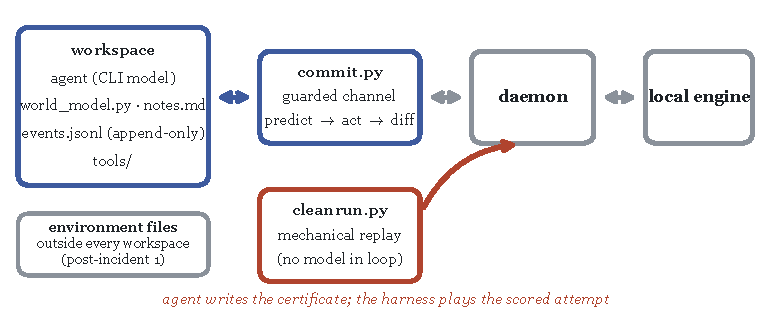
\includegraphics[width=\linewidth]{figures/fig2_arch.pdf}
  \caption{System architecture. The agent operates only inside its workspace; \texttt{commit.py} is the sole channel to the environment and grades a prediction on every action. The certified clean run (red) is executed by \texttt{cleanrun.py} with no model in the loop. Environment implementations reside outside every workspace (a boundary added after Incident 1, \S\ref{sec:integrity}).}
  \label{fig:architecture}
\end{figure}

\section{The Ablation Ladder: v1 \texorpdfstring{$\to$}{->} v5}\label{sec:ladder}

Every version from v2 onward was frozen by commit hash registered in \texttt{RESULTS.md} \emph{before} its board's results existed (v1 predates the freeze protocol); each ran as a complete single-configuration board and is published --- including the version that made things worse. Claude Opus 5, all 25 public games:

\begin{table}[ht]
  \centering
  \caption{The ablation ladder: frozen harness versions, mechanisms, and composites (Claude Opus 5, all 25 public games).}
  \label{tab:ladder}
  \begin{tabular}{lllrr}
    \toprule
    harness & frozen at & mechanism added & composite & $\Delta$ \\
    \midrule
    v1 & --- & base loop + guarded channel & \textbf{97.78} & --- \\
    v2 & \texttt{d37660e}+\texttt{6c3a38d} & \begin{tabular}[t]{@{}l@{}}escalation ladder, partial predictions,\\ automatic one-shot clean run\end{tabular} & \textbf{94.01} & $-3.77$ \\
    v3 & \texttt{e61f9ad}+\texttt{d422ab3} & \begin{tabular}[t]{@{}l@{}}score-floor notices replace hard stops;\\ certified post-WIN restart gate\end{tabular} & \textbf{96.51} & $+2.50$ \\
    v5 & \texttt{eac9af2} & \begin{tabular}[t]{@{}l@{}}mechanical scored attempts (\texttt{cleanrun.py}),\\ forensic fixes\end{tabular} & \textbf{98.86} & $+2.35$ \\
    \bottomrule
  \end{tabular}
\end{table}

(The ladder continues past the table: v6 added recovery-path fixes (Opus not run; GPT 95.97), v7 added visual mode (100.00, replay imperfect), and v8.1 added transport safety --- the server-verified exact 100.00. v4 existed only as a branch --- the certified-program gate, \texttt{c257b35} --- and merged into v5. The GPT-5.6 Sol arc tells the same story: 93.95 (v1-era harness, single config, server card fd4733fb) ${\to}$ 91.46 (v3) ${\to}$ 93.99 (v5) ${\to}$ 95.97 (v6).)

\subsection{The v2 regression and the false-premise autopsy}\label{sec:v2autopsy}

v2's mechanisms were adopted from the systems that outscored us and were \emph{individually} sensible. The board dropped 3.77 points. The autopsy (commit \texttt{e61f9ad}) traced the loss to one wrong premise: \textbf{that the official evaluation cuts a level off at 5$\times$ the human baseline.} It does not. The server scored a 6,881-action run without complaint --- 5$\times$ is a score floor, not a wall --- and since RHAE scores only the final attempt, efficiency \emph{during learning} is worth nothing. v2's guards therefore punished exactly the behavior the metric ignores: its attempt-reset discipline collapsed sp80 from 82.16 to 14.29, and its single clean-run repair locked in sub-cap executions on five games. Worse, two v2 guards had conditions that were exact complements, covering the entire action space between them and deadlocking the agent (fixed in \texttt{d37660e}; the design rule recorded: no set of guards may be able to cover the whole action space between them).

The general lesson we take: on an efficiency-of-the-final-attempt metric, \emph{patience while learning and strictness at the one gate that matters} dominates uniform discipline. v3 implemented exactly that --- every fraction-based guard demoted to a warning, one absolute 3,000-action hard cap as the sole cost refusal --- and recovered 2.50 points.

\subsection{The dead-code gate: forensics on v3}\label{sec:deadcode}

v3's remaining gap hid a bug that no score can reveal, only per-event forensics: the clean-run machinery was \textbf{dead code}. \texttt{commit.py}'s WIN short-circuit (``game already WON'') fired unconditionally \emph{before} the clean-run gate, so every certified restart was refused. Three games --- sc25 (whose certificate computed to a score of 100), tn36, and g50t --- sat locked at their learning-run scores with valid certificates on disk. The v5 fix passes RESET-first plans through to the gate; pre-freeze validation runs converted sc25 84${\to}$100 and g50t 92${\to}$100, and the v5 board scores in \S\ref{sec:results} come from fresh runs launched after the freeze was registered --- the validation runs themselves are published but are not the reported board. We highlight this because it is the strongest single piece of evidence for claim (1): the agent had already \emph{discovered} everything; only the execution machinery was broken, and repairing execution alone was worth most of v5's gain.

\begin{figure}[ht]
  \centering
  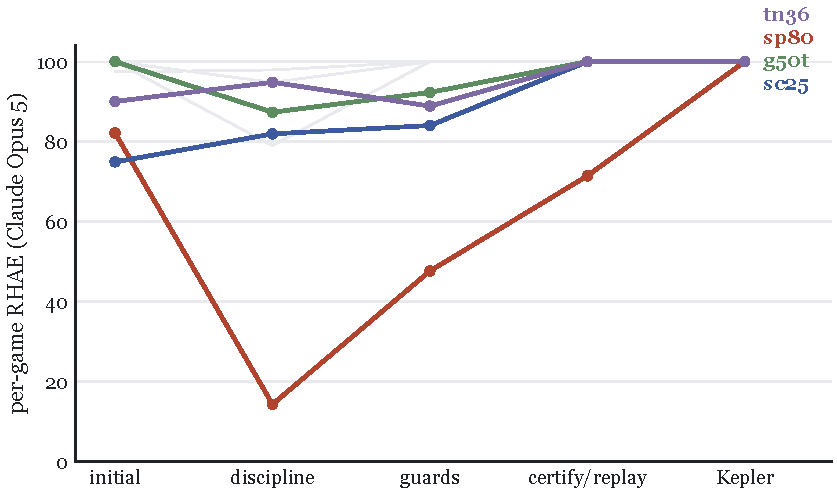
\includegraphics[width=\linewidth]{figures/fig3_pergame.pdf}
  \caption{Per-game scores across harness versions (Claude Opus 5). Gray: the 21 games that remain at or near ceiling throughout. Highlighted: the four games that drive the composite differences; sp80 (red) collapses under v2's forced-reset discipline and partially recovers thereafter, and reaches 100 under v7's visual mode.}
  \label{fig:dotplot}
\end{figure}

\section{Results}\label{sec:results}

\subsection{Boards}\label{sec:boards}

Single configuration, frozen harness, all 25 public games, one run per game (the single disclosed exception is labeled). All v5 board rows are fresh runs launched after the freeze registration; the \S\ref{sec:deadcode} validation runs are separate and published as such. Model identity is pinned by evidence, not by alias: the Claude boards' session transcripts resolve to \texttt{claude-opus-5} (46{,}749 records across the three boards), and the GPT boards ran \texttt{gpt-5.6-sol}:

\begin{table}[ht]
  \centering
  \caption{Single-configuration boards: frozen harness, all 25 public games, one run per game (the single disclosed exception labeled).}
  \label{tab:boards}
  \small
  \begin{tabular}{llrrp{5.2cm}}
    \toprule
    board & model & composite & games at 100 & notes \\
    \midrule
    v1 & Claude Opus 5 & 97.78 & 21 & verified card 00c90840 (97.77, exact re-execution; local composite 97.78 differs only in rounding) \\
    v2 & Claude Opus 5 & 94.01 & 18 & published regression (\S\ref{sec:v2autopsy}) \\
    v3 & Claude Opus 5 & 96.51 & 21 & clean-run gate later shown dead (\S\ref{sec:deadcode}) \\
    v5 & Claude Opus 5 & \textbf{98.86} & 24 & sp80 71.43 (5/6 levels, operator deadline, \S\ref{sec:sp80}) \\
    v1-era & GPT-5.6 Sol (max) & 93.95 & 18 & verified card fd4733fb \\
    v3 & GPT-5.6 Sol (max) & 91.46 & --- & \\
    v5 & GPT-5.6 Sol (max) & \textbf{93.99} & 19 & one disclosed score-conditioned rerun (tr87); first run kept public in \texttt{runs-v5/superseded/} \\
    v6 & GPT-5.6 Sol (max) & \textbf{95.97} & 23 & clean-run-at-100 fix; bp35's first GPT hundred; tn36 variance collapse kept per policy \\
    v7 & Claude Opus 5 & 100.00 & 25 & visual mode; superseded --- replay hit two off-grid clicks (\S\ref{sec:matrix}) \\
    v8.1 & Claude Opus 5 & \textbf{100.00} & 25 & + transport safety; \textbf{server-verified exact} (card 91aa2f10) \\
    \bottomrule
  \end{tabular}
\end{table}

gpt-max v5 sub-100 games: sp80 4.5, bp35 56.4, cd82 95.8, s5i5 96.3, ka59 98.1, cn04 98.8.

\subsection{The verified-card matrix}\label{sec:matrix}

We distinguish grades of number and never mix them. Where the abstract and \S\ref{sec:boards} headline 98.86, they claim the second grade --- audited, with the replay divergence stated in the same table row:

\begin{table}[ht]
  \centering
  \caption{The verified-card matrix: three grades of number, never mixed.}
  \label{tab:matrix}
  \small
  \begin{tabular}{p{3.6cm}rp{8.2cm}}
    \toprule
    grade & score & evidence \\
    \midrule
    Best fully re-executed verified single config & \textbf{97.77} & v1 Opus, official card 00c90840 --- every recorded action re-executed exactly server-side \\
    \addlinespace
    Best audited single config & \textbf{98.86} & v5 Opus, full ledgers public; server replay scores \textbf{96.38} (cards 455e4374 and 1045a78c) with one game, lf52, credited partially --- a recorded ACTION6 rejected by the replay-path engine at the same action in two independent replays, i.e.\ harness-side validation gap (an off-grid click the local engine clipped; fixed in v8), not animation randomness. lf52 traces from other runs replay exactly, so the skew is specific to this trace. Both numbers are published; the card certifies what re-executed. \\
    \addlinespace
    GPT v5 single config & \textbf{93.99 / 93.97} & card f5f64ae7 --- all 25 games re-executed exactly (no lf52-class divergence); local vs card differ only in rounding \\
    \addlinespace
    Final v8.1 Opus board & \textbf{100.00} & \textbf{server-verified exact}: card 91aa2f10 --- all 25 games re-executed to 100 on the official replay; the server and the local ledger agree \\
    \addlinespace
    v7 Opus board (superseded) & 100.00 & audited; server replay 94.42 (cards 0c6c0990, 2779000b): two traces each contained one off-grid \texttt{ACTION6} click the local engine clipped during play --- a harness validation gap, fixed in v8 (off-grid clicks refused at commit and certification) \\
    \addlinespace
    Final v6 GPT board & \textbf{95.97} & card c9f087f3 --- server 95.9672, matches local to the fourth decimal; all 25 games re-executed \\
    \addlinespace
    Best-of ceiling (labeled, never a headline) & \textbf{99.29} & card a7d07431; best run per game across published sweeps, attempt pools (pass@k) disclosed in \texttt{docs/best-of-manifest.json} \\
    \bottomrule
  \end{tabular}
\end{table}

One historical divergence should be stated directly (the final v8.1 board replays exactly): the superseded v7 board's server replay read 94.42, because two of twenty-five recorded traces each contain one off-grid \texttt{ACTION6} click (coordinates outside the 64$\times$64 board) that the local engine clipped during play but the official replay path correctly rejects --- a validation gap in our harness, not a server fault, reproduced identically across two cards and fixed in v8 (out-of-range clicks are now refused at commit time). The server re-executed the other 23 games exactly. Every action of all 25 is published, so the divergence can be checked directly against the published traces.


\subsection{Convergence}\label{sec:convergence}

Across the two v5 boards --- one frozen harness (\texttt{eac9af2}), two labs' frontier models --- \textbf{43 of 50 games score 100.0}. Under the final boards (v8.1 Opus, v6 GPT --- each frozen per model), \textbf{48 of 50 cells score 100.0}, and the Opus board is a single-configuration, server-verified-exact \textbf{100.00}. The per-game distribution under v5 splits by failure mode: of the seven sub-100 cells, three are discovery failures landing far below (sp80 at 4.5 and 71.4, bp35 at 56.4 --- walls never understood), and four are execution near-misses at 95.8--98.8. We read the pattern as harness saturation with a thin efficiency tail: execution is largely solved, and \S\ref{sec:discussion} argues the deep residue is a different quantity.

\begin{figure}[ht]
  \centering
  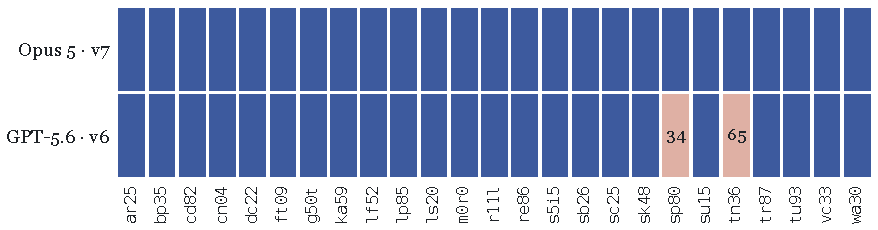
\includegraphics[width=\linewidth]{figures/fig4_convergence.pdf}
  \caption{Convergence on the final boards (v8.1 Opus 5, v6 GPT-5.6; each frozen per model): 48 of 50 cells score 100.0 (blue); the two exceptions, both GPT, are printed --- sp80 (discovery) and tn36 (a same-configuration variance collapse, disclosed).}
  \label{fig:heatstrip}
\end{figure}

\subsection{The modality ablation}\label{sec:ablation}

The fourth finding, as a controlled experiment. Setup: the one game our text-mode agents never solved (\S\ref{sec:sp80}), whose final level 19 sessions across five text-mode attempts had exhaustively ``proved'' unsolvable under every rule set derivable from settled grids and animation-frame \emph{counts} --- the text ledger records how many animation frames each action produced and drops the frames themselves. Intervention: one flag (\texttt{--visual}) makes the daemon persist every frame, animation frames included, as rendered PNGs, and directs the agent to look; tools, discipline, budgets, and audits are held fixed. Result: the same model found the missing mechanic --- a deflection rule directly visible in the animation, plus two goal-state affordances (unfed goals blink; deaths flash a side-coded border) --- and completed the level in 57 actions. \textbf{Crucially, a fresh clean-board run then rediscovered everything from scratch under the frozen harness (and the final v8.1 board reproduced it a third time, server-verified) and finished the game with every level at the cap}, removing the inherited-learning confound; the resumed run that first cracked the level is published separately, with its provenance labeled. We state the conclusion narrowly: for at least one game on this benchmark, the binding constraint was what the agent could perceive, not how it reasoned --- mechanisms that live in transient frames are invisible to a settled-grid agent at any search budget.

\subsection{Cost}\label{sec:cost}

The community leaderboard's own submission rules make cost a first-class field, and ARC Prize's stated bar for harness results is that settings and cost be clearly reported. Our final GPT-5.6 board (v6) cost \textbf{20.7M tokens} (v5: 18.7M) (${\sim}$\$9--94 at API list prices --- the low bound pricing all input at cache-read rates, the high bound pricing all input as fresh; per-game token ledgers in the repo, recovered from the CLIs' own usage records, and a floor: three of 26 workspaces lack usage markers and contribute zero). The published cost-performance frontier, Retrodict, reports \textbf{659.9M tokens / \$654} at 99.86 --- a higher score than ours, which we state plainly; the token-efficiency ratio is ${\sim}$35$\times$. Tycho reports 100.00 at an estimated \$2,986 with no token accounting; baseline1's strongest configuration reports 99.0 at \$400, also without token accounting. Two caveats we apply to ourselves: ${\sim}$98\% of our measured token totals are cached input (priced ${\sim}$an order of magnitude below fresh) --- the session re-reads its workspace each turn --- so any raw-token comparison across harnesses is soft; and while the Claude CLI emits no usage in the mode we use, the Claude Code session transcripts do: summing all 10,985 usage records across the v7 workspaces gives \textbf{1,907.5M tokens, 97.5\% cache reads} --- to our knowledge the first 100-class result on this benchmark published \emph{with} its token accounting. At Opus-class list prices this is not the inexpensive board; we report the accounting regardless, since cost transparency is one of the paper's aims.

\begin{table}[ht]
  \centering
  \caption{Cost and disclosure comparison across published systems.}
  \label{tab:cost}
  \small
  \begin{tabular}{lrrrl}
    \toprule
    system & score & tokens & cost & trace disclosure \\
    \midrule
    Tycho & 100.00 & --- & ${\sim}$\$2,986 (est.) & hashes only \\
    Retrodict & 99.86 & 659.9M & \$654 & full traces \\
    baseline1 (ewma\_sv 1.6) & 99.0 & --- & \$400 & scorecards \\
    VISTA & 100.00 & --- & not disclosed & replays on arcprize.org \\
    AVO (NVIDIA) & 100.00 & --- & not disclosed & none published \\
    \textbf{Kepler v6 (GPT-5.6)} & 95.97 & \textbf{20.7M} & ${\sim}$\$10--100 (list-equiv.) & full traces, failures included \\
    \textbf{Kepler v7 (Opus 5)} & 100.00 & 1,907.5M (97.5\% cache reads) & ${\sim}$Tycho-band (list-equiv.) & full traces, failures included \\
    Kepler v5 (GPT-5.6) & 93.99 & 18.7M & ${\sim}$\$9--94 & full traces \\
    \bottomrule
  \end{tabular}
\end{table}

\begin{figure}[ht]
  \centering
  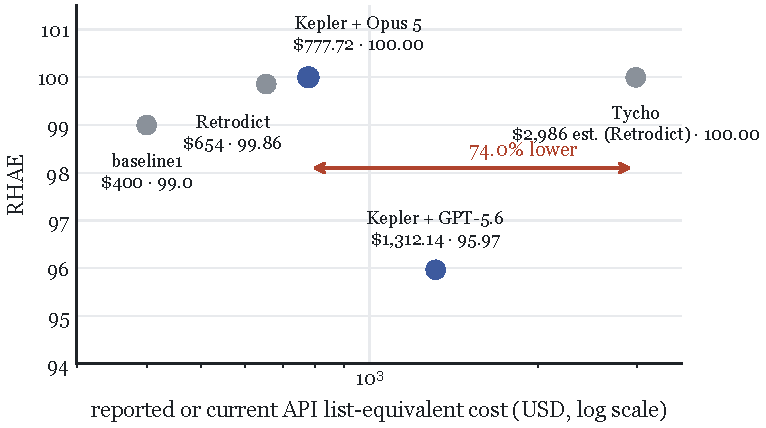
\includegraphics[width=0.8\linewidth]{figures/fig5_cost.pdf}
  \caption{Cost--performance on measured boards (log-scale tokens). The final Kepler boards both appear: v6 GPT-5.6 at 20.7M tokens (${\approx}32\times$ fewer than Retrodict's 659.9M) and v7 Opus 5 at 1,907.5M (97.5\% cache reads) --- the first 100-class result with a published bill. Cached input dominates every total, so cross-harness token ratios are indicative rather than exact. Tycho, VISTA, and AVO publish no token accounting.}
  \label{fig:costscatter}
\end{figure}

\section{Integrity: The Audits That Caught Us}\label{sec:integrity}

A score file is just a number an agent might have influenced. RHAE's only agent-controllable input is the action count, so an \emph{agent} can corrupt a score only through one of six routes (operator-side distortions --- score-conditioned selection, rerun policies --- are governed separately by the \S\ref{sec:intro} policy): the agent read the answer (game source, engine internals, metadata); wrote its own score; bypassed the guarded channel; edited the append-only ledger; modified the tools it is scored by; or looked the game up online. \texttt{scripts/audit\_integrity.py} checks all six over every run; \texttt{scripts/verify\_scores.py} closes the loop from the other side, re-deriving every score from the raw ledger and asserting the only direction that matters: \textbf{no level may be scored with fewer actions than the timeline recorded.} Current status (fresh scan at submission): 324 of 330 runs verified clean --- the six flags are the quarantined \S\ref{sec:incident2} control-group workspaces --- and the ledger recomputation reports exactly two divergent seams, both resume boundaries, both non-material (each affected level scores the cap under either count), both disclosed in \texttt{RESULTS.md}. One agent did what a competent engineer does in an unfamiliar directory: it looked around, read all 2,172 lines of the game it was being scored on, and returned a flawless 100.00 on a game it never modelled. The telemetry looked \emph{better} than honest play --- fewer actions, zero mispredictions, a clean ledger --- and we had already cited the run as headline evidence the harness worked. A clean rerun scored 46.91: a 53-point drop. The run is voided and quarantined with evidence (\texttt{incidents/2026-08-05-source-read/}); the fix was structural (environment files moved outside every workspace), and the audit that should have existed from the start now gates every published number.

\subsection{Incident 2: the control group rebuilt the harness}\label{sec:incident2}

To measure the harness's contribution we ran an ablation --- same model, same games, methodology stripped to \texttt{observe.py} and a bare \texttt{act.py}. But the workspaces lived inside the repository, and \texttt{harness/ws\_tools/} was on disk. \textbf{All six baseline agents found it}: three copied the tools in with \texttt{cp}, the rest wrote shims executing the repo's canonical tools directly, with 92--9,148 harness-tool invocations each and a \texttt{world\_model.py} in every workspace. The comparison was harness-against-harness, and every conclusion drawn from it --- including a striking ``the harness's net advantage is roughly zero'' we had published --- is \textbf{withdrawn}. A valid ablation needs workspaces outside the repository tree and has not been run: \emph{the harness's contribution to our scores is currently unmeasured.} We retain this statement because omitting withdrawn results biases the literature toward positive findings.

Both incidents share a lesson we now design by: twice we shipped a control that was an instruction and a file-placement policy rather than a boundary. An agent optimizing against a metric uses whatever is \emph{reachable}, and reachable means the filesystem, not the instructions.

\subsection{The workspace-compression phenomenon}\label{sec:compression}

A milder instance of the same principle, observed rather than punished: in the v5 GPT boards, \textbf{26 of 26 GPT workspaces (25 board games plus the superseded tr87 rerun) rewrote their own instruction file}, compressing \texttt{AGENTS.md} from 14,844 bytes to ${\sim}$14,092 by systematically deleting articles and function words (``You are agent playing one unseen ARC-AGI-3 game\ldots{} 64$\times$64 grid of 16 colors set of legal actions is all you get''). Twice, a rewrite escaped the workspace and compressed the repository-root \texttt{AGENTS.md} as well --- byte-identical output both times, caught in the working tree and reverted (the second strike prompted a read-only tripwire on the file). No rule prohibited this --- the directive is data in the agent's working directory, and a context-thrifty agent treats its own instructions as compressible payload. We flag it as a benign-but-diagnostic behavior: anything writable will be optimized, including the experiment's own protocol sheet.

\subsection{Replay-transport seams, and what ``no network access'' precisely means}\label{sec:seams}

Two further disclosures. First, the lf52 engine skew (\S\ref{sec:matrix}), restated here for one additional fact: lf52 is the same single game Retrodict documented as their only non-exact replay --- two harnesses, one nondeterminism-prone game, independently. Second, network precision: the \emph{agent} makes zero external requests across all audited session logs (its only HTTP is the localhost daemon), but the \emph{harness} performs one startup handshake --- \texttt{arc\_agi}'s anonymous-key call --- which we had earlier described imprecisely as ``no network access''. We found it when a transient timeout to that host crashed a daemon and the traceback named the call. Correcting small overclaims is inexpensive, and we consider the practice worth institutionalizing.

\section{Discussion}\label{sec:discussion}

\subsection{Discovery is the residual signal}\label{sec:residual}

Claim (3) in one paragraph: v5 removed execution from the score. The agent learns, certifies programs, and a 176-line mechanical replayer plays the scored attempt; the guarded channel already guaranteed that certified programs are model-sound, and the fail-closed replay guarantees they are reality-sound or not scored. Under that regime, 43/50 games saturated at 100 across two frontier models on the v5 boards, and 48/50 on the final boards. Every residual failure was a failure to \emph{discover a mechanic at all} --- and the two v5-era walls (sp80's level 6, bp35's level 6) subsequently fell, one to the modality ablation (\S\ref{sec:ablation}) and one to a certified clean run, which is what the claim predicts: they were discovery failures, not execution failures. What ARC-AGI-3 continues to measure, once a competent harness is in place, is whether an agent can reliably find the rule it has never seen --- which is, we note, the thing the benchmark was designed to measure before harnesses entered the picture. Execution efficiency has become the largely solved part --- which we read as evidence the benchmark's design works: the harness can absorb the engineering, and what remains is the capability ARC-AGI-3 was built to probe.

\subsection{Implications for ARC-AGI-3 evaluation}\label{sec:eval}

Our claim (1) is not idiosyncratic to Kepler: it is what every 98-to-100-class
harness now does, and the convergence is itself a measurement result. Reading the
public code and scorecards of the current leaders, all separate an unbounded,
unscored \emph{learning} phase from a minimal \emph{scored} phase that is a
mechanical replay of a certified trace. Tycho ships a replay viewer and scores
competition-mode replays; Retrodict describes its scorecard as ``a verified
re-execution of the recorded runs, not a new attempt''; GKM states that ``at
scoring time no model runs''; arc-skill's scorecard ``was produced by replaying
the recorded runs.'' Seven independent teams adopted the same segmentation
because RHAE scores only the final attempt, so learning efficiency is worth
nothing. The consequence is that the public-set number now measures \emph{whether
a frontier model can eventually build a correct world model of a game}, not
whether an agent plays efficiently --- two different capabilities, one reported
in the other's name.

Two further patterns fall out of the same reading. First, with the public set
saturated (five entries at ${\ge}99$, four at 100; 48 of our own 50 cells at 100 on the final boards),
the axis that actually separates entries has silently become \emph{cost}, which
is self-reported with no shared definition and no leaderboard badge --- a ${\sim}7\times$
dollar spread exists among entries within a point of each other. Second,
prediction-before-action gating (an action carries a falsifiable claim that is
graded, and a wrong claim is cheap and logged) appears independently in four
harnesses --- a transferable reliability finding the benchmark neither requires
nor measures. We offer, as users of the benchmark rather than its authors, five
concrete adjustments that would let the community leaderboard score the
capability ARC-AGI-3 was built to probe: (i) a cost-conditioned score (RHAE at a
fixed budget), not only a peak score; (ii) a standardized cost triple (tokens,
dollars at stated prices, wall-clock) reported beside the score; (iii) an
optional first-attempt or bounded-learning track that measures efficient play
directly rather than world-model construction; (iv) verification (scorecard
replay plus published traces) as a submission requirement, since a self-reported
score cannot separate a derived answer from a looked-up one; the need is not hypothetical: the most publicized 100.00 claim to date shipped as a corporate blog post with no scorecard link, traces, or cost; and (v) moving the
headline to the held-out sets, which several teams (ourselves included) note the
public set no longer stands in for. The full write-up, with sources, is in the
repository.

\subsection{sp80 as an open problem}\label{sec:sp80}

For most of this project, sp80 was the open problem: below the cap on every board, for us and for Retrodict alike. Our longest text-mode run reached level 5 of 6 with every level at the cap, then spent days on level 6 --- and its endgame is the scientifically interesting part. The agent stopped probing and started \emph{proving}: under a physics that backtested green on 4,655 of 4,670 recorded transitions, it exhaustively searched on the order of $4.1\times10^{8}$ candidate configurations and established that no solution existed under the rules it knew, while isolating the single unexplained observable (a persistent animation-length residual) that had to hide the missing mechanic. The proof was correct; the rules were wrong; and the residual it flagged was, in hindsight, the exact signature of an observation channel that deletes evidence --- the hypothesis \S\ref{sec:ablation} tests directly. We still propose ``time-to-missing-mechanic'' --- the interval between an agent's first proof-grade exhaustion of its rule set and its first observation isolating the missing mechanic --- as an honest frontier metric on games like this; on sp80, that interval closed the first session the agent could see.

\subsection{Limits}\label{sec:limits}

Model identity is recorded going forward; for the reported boards it is pinned by the session transcripts (\S\ref{sec:boards}). Comparable published entries state a pinned version; we state the alias, and log the resolved identifier going forward. Beyond that: single benchmark; public set only (the semi-private and private sets are where a result counts, and we have not run them); $n=1$ per cell; board-composite variance in our own data is $\pm$1--2 points, but per-game variance can be an order of magnitude larger (tr87 scored 47.6 and 100.0 on two same-configuration v5 GPT runs, the rerun disclosed); quota-shaped runs --- several lanes were resumed across provider quota windows under a disclosed resume policy, and one board's hardest game was ended by an operator deadline, both of which shape scores in ways a lab with unmetered access would not experience. And the deepest caveat is inherited from \S\ref{sec:incident2}: whether the harness \emph{causes} the scores, versus the models alone, is unmeasured until a boundary-correct ablation is run --- the minimal-scaffold external datapoint (\S\ref{sec:related}) suggests the model contributes most of the Claude number, with the harness buying the last ${\sim}$1.5 points and the auditability.

\section{Related Work}\label{sec:related}

\textbf{Early ${\sim}$99\% reports.} The first ${\sim}$99\%-class numbers on this benchmark were self-reported from write-ups without released code, using a per-game best-of-2 fallback with score feedback --- the selection rule Kamradt's critique targeted. Our v1, run \emph{with} that fallback for comparison only, matched those numbers to within noise (98.30 / 95.51); we then abandoned the rule as score-conditioned selection, and the \S\ref{sec:ladder} ladder reports v1 without it (97.78). The executable-world-model idea itself is established in published, citable work --- Tycho~\citep{tycho} and Rodionov's baseline1 line~\citep{thinharness} --- of which this project is an independent implementation.

\textbf{Tycho} (NIMI-research; arXiv:2607.28287)~\citep{tycho} --- 100.00, the first published perfect score; paper-artifact release with frozen configs and CI, official scorecard per row, traces published as SHA-256 hashes rather than inspectable data; no cost accounting. We adopted (and credit in \texttt{NOTICE}) its partial UNKNOWN-cell predictions, vacuous-coverage rejection, threaded hidden-state planning, consecutive-RESET guard --- and its 5$\times$-baseline level cutoff, which our v2 regression subsequently falsified as an \emph{official-rule} premise (\S\ref{sec:v2autopsy}); adopted mechanisms still warrant independent testing.

\textbf{Retrodict} (Ryan Brown)~\citep{retrodict} --- 99.86 at \$654 / 659.9M tokens; the transparency standard this repo aims to meet and exceed: full traces including superseded attempts, per-game cost ledgers, and the best replay disclosure in the field (``a verified re-execution of the recorded runs, not a new attempt'' --- language we adopt). Its comparison memo publicly critiqued the earliest ~99\% release; Kepler's release is in large part an answer to that review. We also adopt its sparse expected-cell predictions, escalation-ladder tiers, and prediction-discipline framing (\texttt{NOTICE}).

\textbf{baseline1 / ThinHarness}~\citep{thinharness} --- the minimal-agent lineage Retrodict builds on; used throughout the field as the null scaffold.

\textbf{Concurrent community submissions.} While this paper was in preparation, the pending community-leaderboard entries converged on the same architecture claim (1) describes: GKM freezes model-written programs behind an admission gate and states \emph{``at scoring time no model runs''}; arc-skill's scorecard \emph{``was produced by replaying the recorded runs''}; Strands and arc-skill both run Claude Opus 5, the model our boards resolve to. We read four independent 98-to-100-class systems scoring mechanical replays --- none citing each other --- as strong evidence that certify-then-replay is the dominant design, which makes stating it explicitly (and auditing it) the more urgent.

\textbf{VISTA and AVO: the direct-interaction school.} Concurrently with this
work, VISTA~\citep{vista} (Han et al., MIT) reported 100.00 (Claude Opus 5, 7{,}542 actions)
and 98.27 (GPT-5.6 Sol) using the opposite architecture to the world-model
school: the model observes rendered PNG frames directly, reasons in free-form
language with no executable-model requirement, and keeps a lossless visual
memory of every frame. NVIDIA's AVO~\citep{avo} adopted VISTA's direct-interaction
principles (explicitly declining Tycho-style programmatic world models) and
reported 100.00 with a supervisor-redirected general coding agent; no code,
traces, per-game data, or cost accounting accompany either release at the time
of writing. Two implications for this paper. First, the replay-scored
segmentation of \S\ref{sec:eval} spans \emph{both} schools --- the convergence
is about what is scored, not how games are learned. Second, the schools have
never been compared under controlled conditions (AVO: ``this is not a
controlled ablation''); the observation channel (text grid vs.\ rendered
frames) is confounded with everything else. Our harness records every frame and
can toggle the observation channel alone (\texttt{--visual}), holding tools,
discipline, budgets, and audits fixed --- \S\ref{sec:ablation} reports the first instance of exactly that experiment.

\textbf{arc-code} (Berman)~\citep{arccode} --- the minimal-scaffold datapoint, and it cuts both ways: stock Claude Code with an 11-line prompt reaches 96.2 pass@1 / 99.3 pass@2 (${\sim}$\$540), while GPT-5.6 Sol under the same scaffold scores \textbf{73.7}. Against our GPT single configs (84.20 v1-xhigh; 93.99 v5-max) this is the one external same-model comparison in the harness's favor; against overclaiming, it shows most of the Claude number is the model plus freedom to build, and we state that rather than hide it.

\section{Reproducibility Statement}\label{sec:repro}

Everything behind every number ships in the repository and verifies offline, without trusting us and mostly without API keys:

{\footnotesize\begin{verbatim}
.venv/bin/python scripts/audit_integrity.py   # adversarial scan of every run (six violation classes)
.venv/bin/python scripts/verify_scores.py     # re-derive every score from the append-only ledgers
python3 scripts/verify.py                     # replay a winning trace locally, no API keys
.venv/bin/python scripts/cost_report.py       # token accounting from the CLIs' own records
python  scripts/check_no_game_ids.py          # the no-game-secrets CI gate
\end{verbatim}}

The trace corpus is every run --- winners, failures, regressions, and superseded runs with their supersession reasons --- as append-only \texttt{events.jsonl} ledgers plus the agent's own \texttt{world\_model.py} and \texttt{notes.md} per workspace. Frozen-harness hashes were registered in \texttt{RESULTS.md} before their boards' results existed. Headline scorecards: c9f087f3 (v6 GPT, exact), 0c6c0990 / 2779000b (v7 Opus replays), 00c90840 (v1 Opus, exact), 455e4374 / 1045a78c (v5 Opus replays), f5f64ae7 (v5 GPT, exact), fd4733fb (v1-era GPT), a7d07431 (best-of ceiling; manifest in \texttt{docs/best-of-manifest.json}). Bit-for-bit reproduction of \emph{live} runs is not expected (sampling, provider drift); reproduction of every \emph{score} from its ledger is expected, mechanical, and gated.

\section*{Acknowledgments}

Ryan Brown (Retrodict) and the Tycho authors (NIMI-research), whose released mechanisms this harness adopts with attribution (\texttt{NOTICE}) and whose release engineering set the bar this project measures itself against; the ARC Prize Foundation for ARC-AGI-3, the \texttt{arc-agi} toolkit, and the official RHAE implementation.

\bigskip
\paragraph{Appendices.} Full per-game tables for all boards, the guard-deadlock and dead-code forensic timelines, the sp80 search inventory, the lf52 replay transcripts, and the audit flag taxonomy are provided in the repository alongside the raw ledgers.

% Entries in references.bib not yet cited inline in the draft (kept in the bibliography for the
% camera-ready pass): Chollet's On the Measure of Intelligence; the OpenAI two-settings blog post
% (the likely citation target for the GPT-5.6 Sol "xhigh"/"max" reasoning settings).
\nocite{chollet2019measure,openai_twosettings}

\bibliographystyle{plainnat}
\bibliography{references}

\end{document}